\newpage
\section{Theoretische Grundlagen} \label{infos}
\todo{Einleitung Grundlagen schreiben}

\subsection{Neuronale Netzwerke}
In den letzten Jahren gab es eine Vielzahl von beeindruckenden Fortschritten und Leistungen durch Computersysteme, die durch die Allgemeinheit unter dem Begriff \ac{KI} zusammen gefasst werden. So konnte zum Beispiel AlphaGo einen der weltweit besten Spieler in dem Brettspiel Go schlagen und das System DeepFace ist in der Lage, menschliche Gesichter nahezu auf menschlichen Niveau erkennen zu können.\footcites[Vgl.][]{spiegelGoogleComputerAlphaGo2016}\footcite[Vgl.][]{taigman2014deepface}

Systeme die als \ac{KI} bezeichnet werden, sind häufig in der Lage, Aufgaben zu bewältigen die bisher ausschließlich durch das menschliche Gehirn erledigt werden konnten. Neben den oben genannten Beispielen zählt hier auch das Erkennen von Bildern oder Sprache dazu. Damit Computer diese Aufgaben erledigen können, haben Wissenschaftler sich vom menschlichen bzw. biologischen Gehirn inspirieren lassen. Systeme die auf dieser Grundlage basieren und einige der Vorgehensweisen des Gehirnen imitieren, werden als \ac{NN} bezeichnet.

\subsubsection{Aufbau}
Die grundlegenden Bausteine von \ac{NN} sind Perceptron und wurden 1958 von Rosenblatt beschrieben.\footcite[Vgl.][]{rosenblattPerceptronProbabilisticModel1958} Als Grundlage verwendete er hierbei unter anderem die Arbeit von McCulloch und Pitts.\footcite[Vgl.][]{mccullochLogicalCalculusIdeas1943}

\tikzset{%
  neuron missing/.style={
    draw=none, 
    scale=3,
    text height=0.333cm,
    execute at begin node=\color{black}$\vdots$
  },
}

\begin{figure}[H]
	\centering
	\begin{tikzpicture}[x=1.5cm, y=1.5cm,  >=stealth]
        \tikzstyle{unit}=[draw,shape=circle,minimum size=1.2cm]
        \tikzstyle{weight} =[draw, shape=rectangle, minimum size=.8cm]


        \node[unit](x1) at (0,3.5){$I_1$};
        \node[unit](xn) at (0,1.5){$I_{N}$};
        \node(dots) at (0,2.5){\vdots};
        \node[unit](bias) at (0,0){$b$};

        \node[weight](w1) at (2,3){$w_1$};
        \node[weight](wn) at (2,1.5){$w_n$};
        \node[weight](wb) at (2,0.5){$w_b$};

        \node[unit](wSum) at (4,1.5){$\sum$};

        \draw[->] (bias) -- (wb);
        \draw[->] (x1) -- (w1);
        \draw[->] (xn) -- (wn);
        \draw[->] (wb) -- (wSum);
        \draw[->] (w1) -- (wSum);
        \draw[->] (wn) -- (wSum);

        \draw [->] (wSum) -- ++(1,0)
        node [above, midway] {};
        
        \end{tikzpicture}
	\caption[]{Darstellung eines Perceptron}
    \label{fig:perceptron}
    Quelle: Eigene Darstellung, 2020
\end{figure}

Ein Perceptron kann zwischen $1$ und $n$ Eingangssignalen sowie einen negativen Bias Term\footnote{Einige Defintionen schreiben nicht vor, dass der Bias negativ sein muss. Stattdessen wird dieser im weiteren Vorgehen subtrahiert statt summiert zu werden} $b$ erhalten und hieraus ein Ausgangssignal - auch Aktivierung genannt - erzeugen. Für das Ausgangssignal werden alle Eingangssignale jeweils mit einem eigenen - als Gewicht bezeichneten - Faktor multipliziert (siehe Abbildung \ref{fig:perceptron}). Die Ergebnisse werden anschließend zusammen mit dem Bias summiert. Ist die Summe kleiner oder gleich $0$, ist der Ausgangswert ebenfalls $0$, ansonsten beträgt der Ausgangswert $1$. Der Bias stellt also den Schwellwert dar, denn die gewichtete Summe überschreiten muss, damit das Ausgangssignal $1$ lautet. 

Es ist möglich, ein Perceptron um eine Aktivierungsfunktion zu ergänzen, sodass das Ausgabesignal reelle Werte annehmen kann. Diese Erweiterung des Perceptron wird als Neuron bezeichnet. Weit verbreitet ist die Verwendung der Sigmoid Funktion (siehe Gleichung \ref{eq:sigmoid}). Bei der Anwendung einer Aktivierungsfunktion, häufig mit $\sigma$ dargestellt, wird die gewichtete Summe $z$ in die gewählte Funktion gegeben und das Ergebnis stellt das Ausgangssignal des Neuron da (siehe Gleichung \ref{eq:outputNeuron}).

\begin{equation} \label{eq:sigmoid}
    \sigma (z) =  \frac{1}{1+e^{-z}}
\end{equation}

\begin{equation} \label{eq:outputNeuron}
    a = \sigma (\sum_{i}{x_i w_i + b})
\end{equation}

Neben der Sigmoid Funktion werden in modernen \ac{NN} häufig die ReLu Funktion (Gleichung \ref{eq:ReLU}) oder die tanh Funktion (Gleichung \ref{eq:tanh}) verwendet. Alle drei werden in Abbildung \ref{fig:activationfunctions} gegenüber gestellt. Es ist zu erkennen, dass sowohl bei der Sigmoid Funktion, als auch bei der ReLU Funktion die untere Grenze des Wertebereichs bei $0$ liegt. Bei der tanh Funktion, liegt diese bei $-1$. Außerdem haben nur die Sigmoid- und tanh Funktion eine obere Grenze - beide 1 - definiert. ReLU kann jeden Wert größergleich $0$ annehmen.

\begin{equation} \label{eq:ReLU}
    ReLU(z) = max(0,z)
\end{equation}

\begin{equation} \label{eq:tanh}
    \tanh(z) = \frac{\sinh(z)}{\cosh(z)} = \frac {e^z - e^{-z}} {e^z + e^{-z}}
  = \frac{e^{2z} - 1} {e^{2z} + 1}
\end{equation}

\begin{figure}[H]
    \centering
    \caption[]{Darstellung der Sigmoid-, ReLU- und tanh Funktion}
	\label{fig:activationfunctions}
    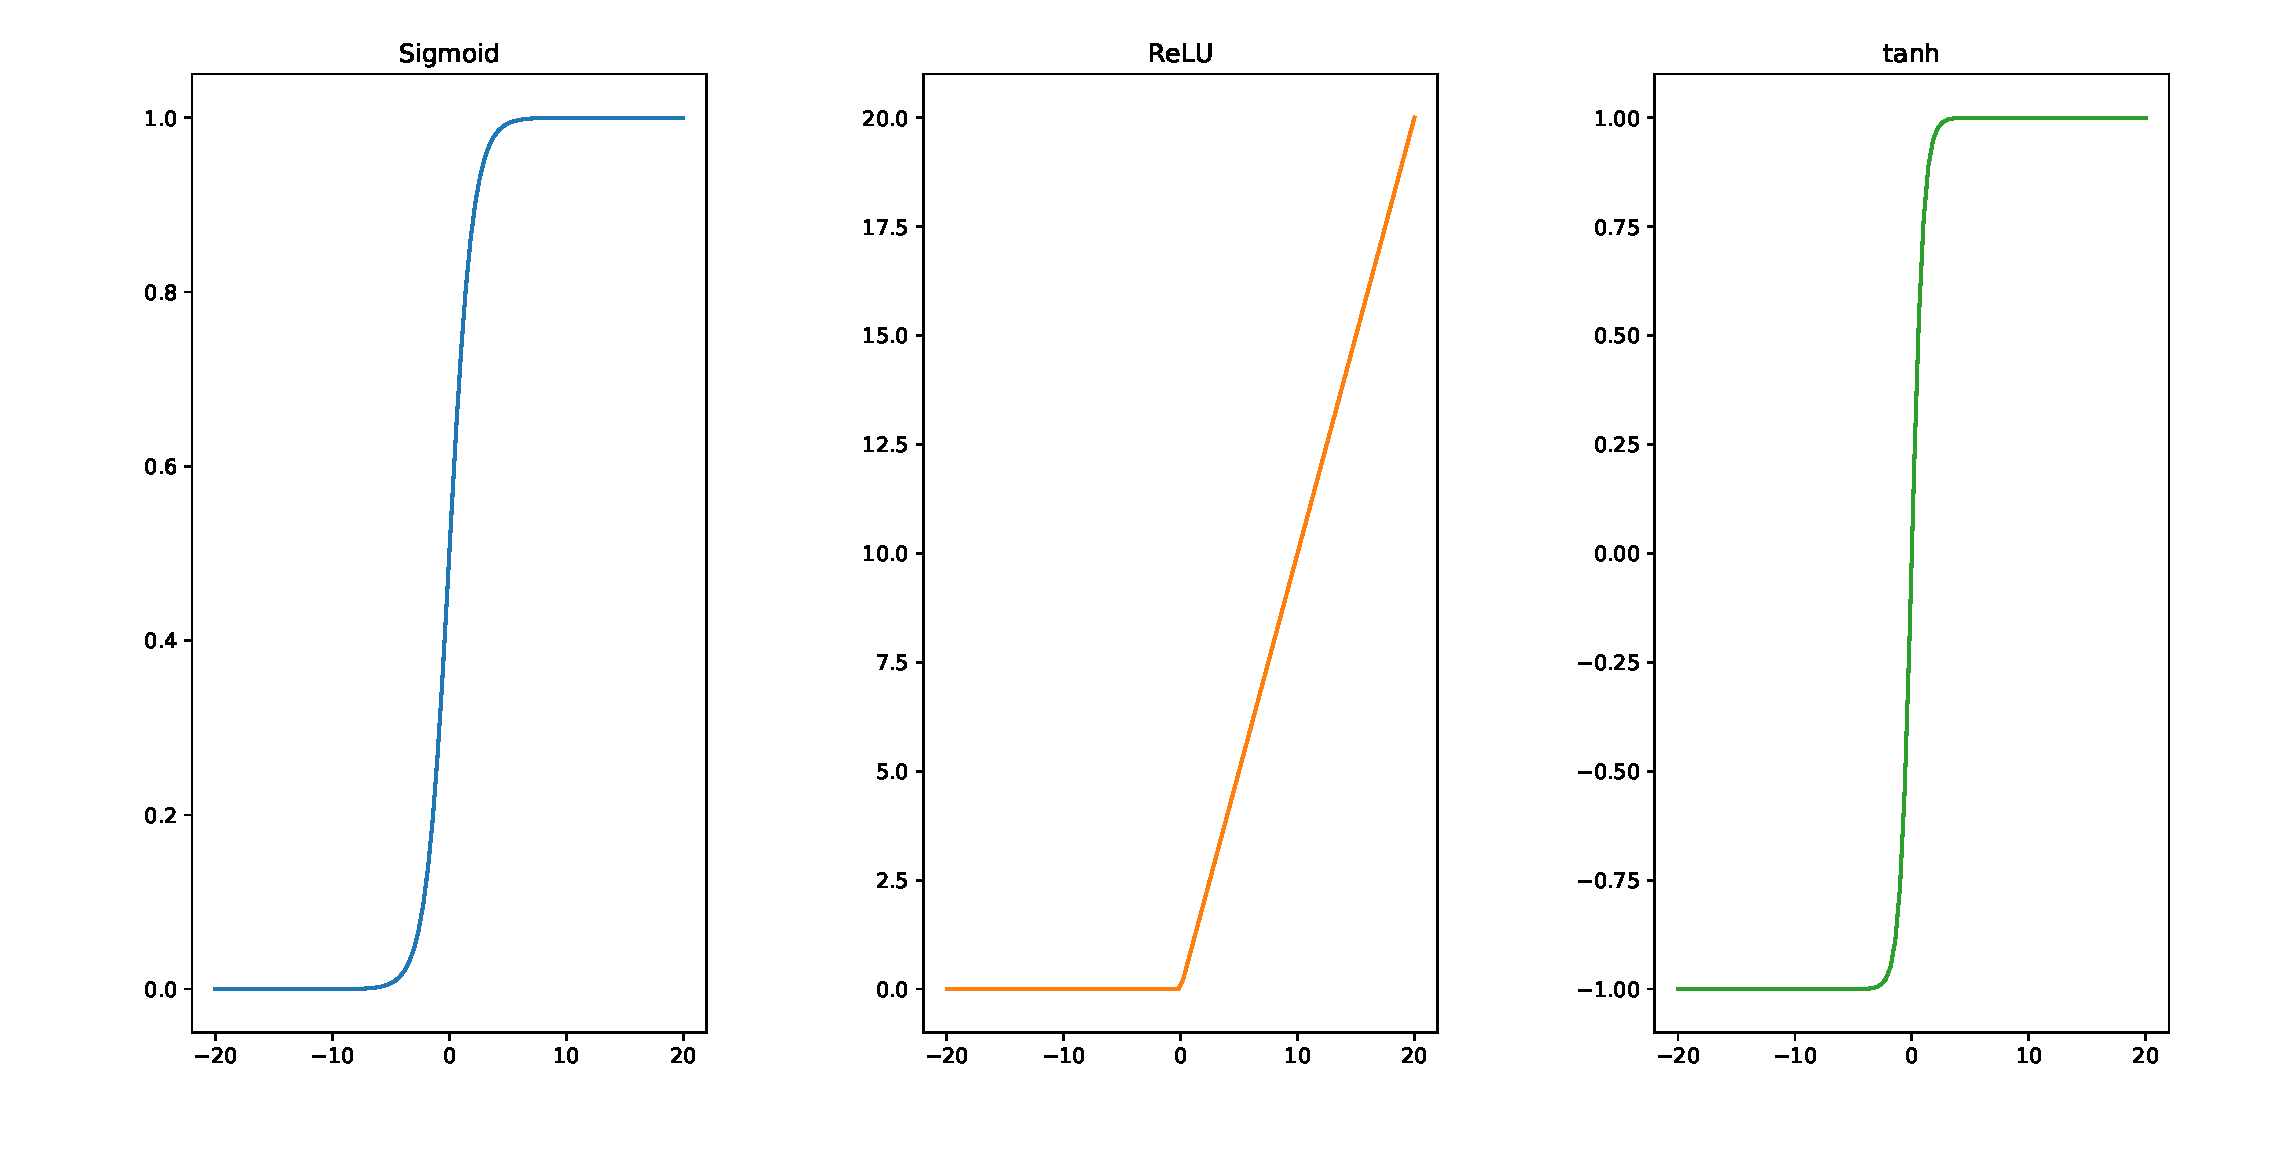
\includegraphics[width=1\textwidth]{activationfunctions.eps}
    Quelle: Eigene Darstellung, 2020
\end{figure}

Ein \ac{NN} besteht aus mehreren, verschalteten Neuronen. Diese werden in Layern angeordnet, welche typischerweise mit $1$ bis $N$ durchnummeriert werden. Layer 1 wird außerdem als Input Layer bezeichnet, da dieser die einzelnen Eingangswerte in das \ac{NN} darstellt. Layer N wiederum wird als Output Layer bezeichnet, da er das Ergebnis des \ac{NN} ausgibt. Alle Layer dazwischen (1 < $l$ < N) werden als Hidden Layer bezeichnet, da von außen weder direkt auf die Eingangssignale der Neuronen in diesen Layern Einfluss genommen werden kann, noch die Ausgabesignale dieser direkt ersichtlich sind. Jeder Layer kann dabei eine unterschiedliche Anzahl von Neuronen enthalten. Eine allgemeine Darstellung eines \ac{NN} mit drei Layern ist in Abbildung \ref{fig:multilayer-perceptron} dargestellt.

\tikzset{%
  every neuron/.style={
    circle,
    draw,
    minimum size=1.2cm
  },
  neuron missing/.style={
    draw=none, 
    scale=3,
    text height=0.333cm,
    execute at begin node=\color{black}$\vdots$
  },
}

\begin{figure}[H]
	\centering
	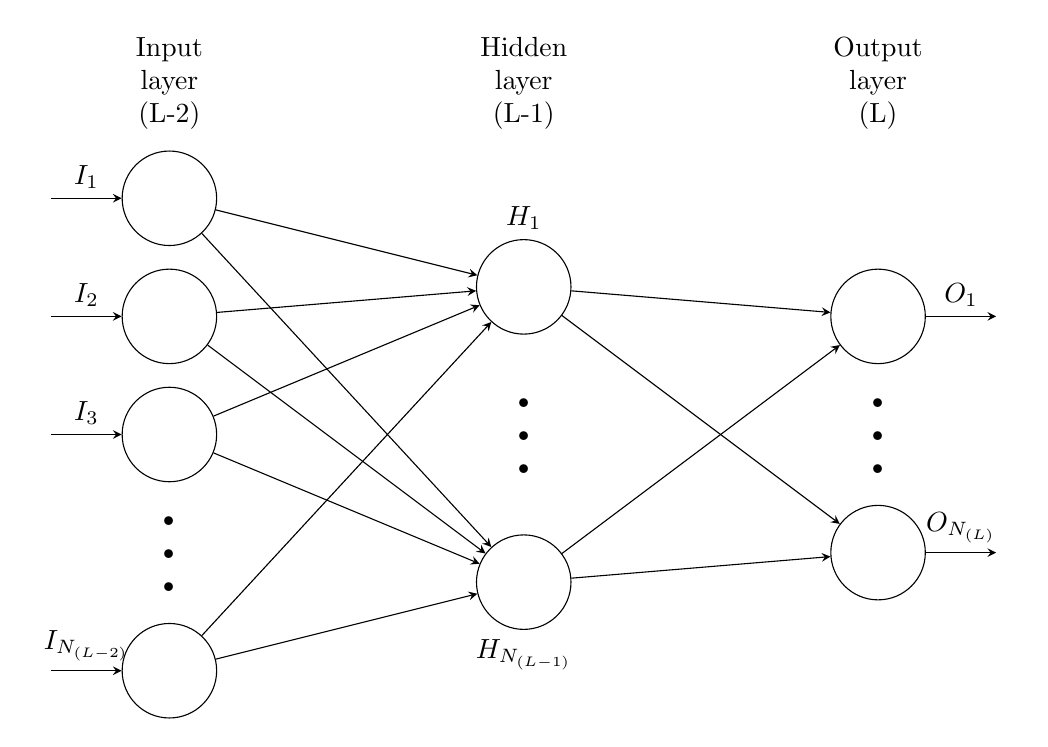
\begin{tikzpicture}[x=1.5cm, y=1.5cm,  >=stealth]

        \foreach \m/\l [count=\y] in {1,2,3,missing,4}
          \node [every neuron/.try, neuron \m/.try] (input-\m) at (0,2.5-\y) {};
        
        
        \foreach \m [count=\y] in {1,missing,2}
          \node [every neuron/.try, neuron \m/.try ] (hidden-\m) at (3,2-\y*1.25) {};
        
        \foreach \m [count=\y] in {1,missing,2}
          \node [every neuron/.try, neuron \m/.try ] (output-\m) at (6,1.5-\y) {};
        
        \foreach \l [count=\i] in {1,2,3}
          \draw [<-] (input-\i) -- ++(-1,0)
            node [above, midway] {$I_\l$};
        \draw [<-] (input-4) -- ++(-1,0)
            node [above, midway] at (input-4) {$I_{N_{(L-2)}}$};
        
        \node [above] at (hidden-1.north) {$H_1$};
        \node [below] at (hidden-2.south) {$H_{N_{(L-1)}}$};
        
        
        \draw [->] (output-1) -- ++(1,0)
        node [above, midway] {$O_1$};
        \draw [->] (output-2) -- ++(1,0)
        node [above, midway] {$O_{N_{(L)}}$};
        
        \foreach \i in {1,...,4}
          \foreach \j in {1,...,2}
            \draw [->] (input-\i) -- (hidden-\j);
        
        \foreach \i in {1,...,2}
          \foreach \j in {1,...,2}
            \draw [->] (hidden-\i) -- (output-\j);
        
        %\foreach \l [count=\x from 0] in {Input, Hidden, Ouput}
        \node [align=center, above] at (0*2,2) {Input \\ layer \\ (L-2)};
        \node [align=center, above] at (1.5*2,2) {Hidden \\ layer \\ (L-1)};
        \node [align=center, above] at (3*2,2) {Output \\ layer \\ (L)};
        
        \end{tikzpicture}
	\caption[]{Allgemein Darstellung eines Neural Network mit 3 Layern}
    \label{fig:multilayer-perceptron}
    Quelle: Eigene Darstellung, 2020
\end{figure}



\subsubsection{Gradient Descent}
Im Rahmen des Lernprozesses eines \ac{NN} werden die Gewichte und Bias der einzelnen Perceptron regelmäßig aktualisiert. Dabei liegt das Ziel darin, durch die Optimierung dieser Faktoren den Fehler des \ac{NN} bei der Vorhersage zu minimieren.

Um diesen Fehler bestimmen zu können, wird eine Verlustfunktion angewendet. Ein einfaches Beispiel einer Verlustfunktion basiert auf der mittleren quadratischen Abweichung.

\begin{equation} \label{eq:mse}
    L(w,b) = \frac{1}{2} \sum (y-\hat{y})^2
\end{equation}

In Gleichung \ref{eq:mse} werden die Gewichte mit \textit{w} und die Bias mit \textit{b} bezeichnet. Zusätzlich werden die wahren Klassen durch \textit{y} und die Ausgabe des \ac{NN} durch \textit{\^{y}} dargestellt. \todo{Prüfen ob variablen konsistent verwendet werden}


Um den Fehler des \ac{NN} zu minimieren, muss der globale Tiefpunkt der Verlustfunktion bestimmt werden. Bei Funktionen mit einer Vielzahl von Parametern, ist es zu komplex, diese Aufgabe analytisch zu lösen. \textit{\ac{GD}} stellt einen iterativen Prozess dar, sich dem nächsten Minimum zu nähern. Bildlich kann dieser Vorgang mit einem Wanderer, der vom Gipfel eines Berges absteigen möchte, verglichen werden. Geht dieser von seinem aktuellen Standpunkt ein paar Schritte in die entgegengesetzte Richtung der steilsten Stelle am Berg und wiederholt diesen Vorgang immer wieder, wandert er immer weiter ins Tal. Betrachtet man Abbildung \ref{fig:quadLoss}, würde der Wanderer in einem der braunen Quadrate beginnen und sich Schritt für Schritt tiefer bis zum blauen Bereich vorarbeiten. 

Mathematisch gesehen kann dies als eine Funktion \textit{L(v)} gesehen werden, wobei \textit{v} eine beliebige Anzahl von Parametern darstellt. Für eine bessere Übersichtlichkeit, wird im folgendem mit zwei Parametern, \textit{v\textsubscript{1}} und \textit{v\textsubscript{2}} gerechnet.

\begin{figure}[H]
    \centering
    \caption[]{Beispiel quadratische Verlustfunktion mit den Parametern v\textsubscript{1} und v\textsubscript{2}}
	\label{fig:quadLoss}
    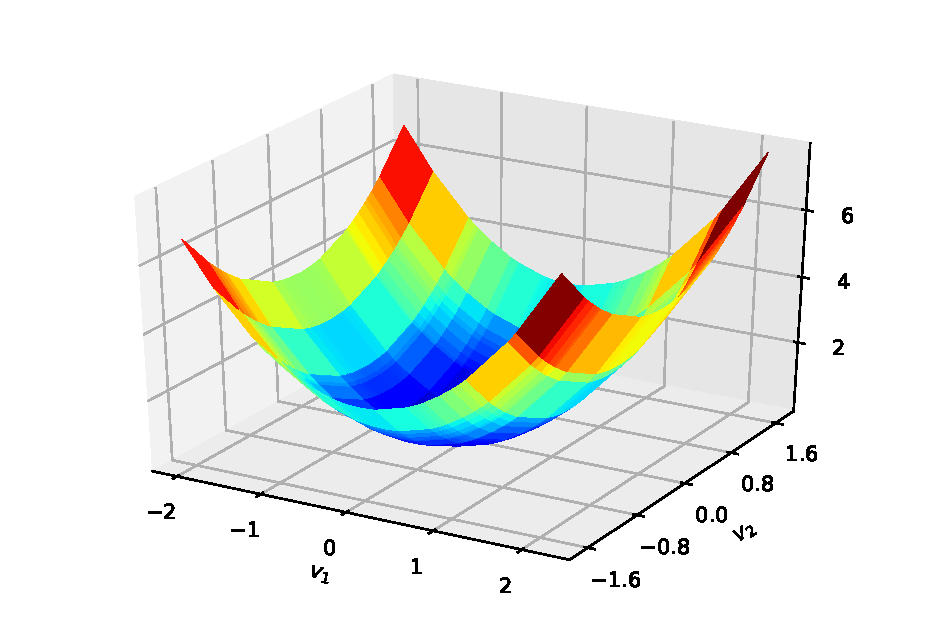
\includegraphics[width=1\textwidth]{quadratic_loss_function.eps}
    Quelle: Eigene Darstellung, 2020
\end{figure}

\begin{equation} \label{eq:deltaL}
    \Delta L \approx \frac{\partial L}{\partial_{v1}} \Delta v_{1} + \frac{\partial L}{\partial_{v2}} \Delta v_{2}
\end{equation}

In Gleichung \ref{eq:deltaL} wird die Funktion $\Delta$L als Summe der partiellen Ableitungen von \textit{v\textsubscript{1}} und \textit{v\textsubscript{2}} definiert. Die hierdurch erhaltenen Gradienten zeigen in die Richtung der größten Änderungen von \textit{v\textsubscript{1}} beziehungsweise \textit{v\textsubscript{2}} .

Fasst man die Parameter \textit{v\textsubscript{1}} und \textit{v\textsubscript{2}} und die partiellen Ableitungen jeweils in einem Vektor zusammen (Gleichung \ref{eq:vector1} und \ref{eq:vector2}), kann Gleichung \ref{eq:deltaL} zu Gleichung \ref{eq:vereinfachung1} umgeformt werden. $\Delta$v kann hierbei als der Vektor der Veränderung der Parameter gesehen werden.

\begin{equation} \label{eq:vector1} 
    \Delta v \equiv \binom{\Delta v_{1}}{ \Delta v_{2}}
\end{equation}

\begin{equation} \label{eq:vector2}
    \nabla L \equiv (\frac{\     L}{\partial_{v1}},  \frac{\partial L}{\partial_{v1}})^{T}
\end{equation}

\begin{equation} \label{eq:vereinfachung1}
    \Delta L \approx \nabla L \cdot \Delta v
\end{equation}

Um den Gesamtverlust zu reduzieren, muss der Vektor $\Delta$v in jedem Durchgang aktualisiert werden. Durch den Gradienten ist die Richtung der größten Änderung vom aktuellen Punkt der Funktion aus bekannt. Da der Gesamtverlust minimiert werden soll, muss in die entgegengesetzte Richtung des Gradienten gegangen werden. Dessen Wert wird also negiert. Außerdem muss eine positive Schrittweite bestimmt werden, die skaliert wie Weit in die Gegenrichtung des Gradienten gegangen wird. Diese wird als \textit{Learning Rate} und häufig mit $\alpha$ bezeichnet. Gleichung \ref{eq:learningRate} zeigt, wie die Veränderung der Parameter, $\Delta$v, mittels $\alpha$ skaliert und das Ergebnis negiert wird.

\begin{equation} \label{eq:learningRate}
    \Delta v = -\alpha \nabla L
\end{equation}      

Wird Gleichung \ref{eq:learningRate} in Gleichung \ref{eq:vereinfachung1} eingesetzt und umgeformt, erhält man Gleichung \ref{eq:finalGradDes}. Da  $\nabla L^2$ und $\alpha$ jeweils positiv sind, ist sichergestellt, dass die vorgenommene Veränderung negativ ist. Dies bedeutet, dass der Verlust mit jedem Durchgang verringert wird, das \ac{NN} also besser wird. Anzumerken ist hierbei noch, dass das Minimum bei einer zu groß gewählten \textit{Learning Rate} überschritten werden kann. Dies würde dazu führen, dass man den Tiefpunkt überschreitet und wieder ein Stück hoch geht. Außerdem kann das erreichte Minimum ein lokales und nicht globales Minimum sein. Dies ist abhängig vom Startpunkt, da der negierte Gradient immer zum nächstgelegenen Minimum führt.

\begin{equation} \label{eq:finalGradDes}
    \Delta L \approx -\alpha \nabla L \cdot  \nabla L =  -\alpha \nabla L^2
\end{equation}

Ersetzt man \textit{v\textsubscript{1}} und \textit{v\textsubscript{2}} durch \textit{w} und \textit{b}, ist die Berechnung der neuen Werte für die Gewichte \textit{w\textsubscript{j}} und Bias \textit{b\textsubscript{j}} wie in den Gleichungen dargestellt \ref{eq:updateW} und \ref{eq:updateB} definiert.
\begin{equation} \label{eq:updateW}
    w_{j} \rightarrow w_{j}^{'} = w_{j} - \alpha \frac{\partial L}{\partial w_{j}}
\end{equation}

\begin{equation} \label{eq:updateB}
    b_{j} \rightarrow b_{j}^{'} = b_{j} - \alpha \frac{\partial L}{\partial b_{j}}
\end{equation}

\textit{\ac{GD}} betrachtet alle Beispiele im Trainingsdatensatz, bevor die Gewichte und Bias das erste Mal angepasst werden. Da dies  besonders bei großen Trainingsdatensätzen sehr zeit- und rechenintensiv ist, wird bei diesen Datensätzen häufig \ac{SGD}\footcite[Vgl. ][S. 400 ff.]{robbinsStochasticApproximationMethod1951}  angewendet. Bei \ac{SGD} werden die Anpassungen bereits nach einem oder einer Gruppe von Beispielen aus dem Datensatz durchgeführt. Dies hat zwar den Nachteil, dass die Optimierung der Verlustfunktion schlechter sein kann als bei \ac{GD}, allerdings konvergiert \ac{SGD} meistens schneller.

\subsubsection{Backpropagation}

Wie im letzten Abschnitt beschrieben, müssen für die Anwendung von \ac{GD}  $\frac{\partial L}{ \partial w}$ und  $\frac{\partial L}{ \partial b}$ berechnet werden. Rumelhart et al. haben für eine schnelle und effiziente Berechnung dieser im Jahr 1986 den Backpropagation Algorithmus vorgeschlagen.\footcite[Vgl. ][S. 533 ff.]{rumelhart1986learning} Dieser stellt eine erweiterung der Delta-Regel auf \ac{NN} mit mehr als zwei Schichten dar.\todo[]{Quelle einfügen} Die Grundidee besteht darin, den Fehler des \ac{NN} auf die einzelnen Gewichte und Bias innerhalb des \ac{NN} zurückzuführen, so dass diese angepasst werden können. Im folgenden wird primär auf die Gewichte eingegangen, da die Berechnung für einen Bias als einfachere Form der Rechnung für Gewichte angesehen werden kann. Formuliert man die Grundidee für die Gewichte um, stellt sich die Frage, in wie sehr sich der Fehler des \ac{NN} ändert, wenn das Gewicht $w_{jk}$ angepasst wird (siehe Gleichung \ref{eq:defDeltaEdef})

\begin{equation} \label{eq:defDeltaEdef}
    \frac{\partial E}{ \partial w_{jk}}
\end{equation}

\begin{figure}[H]
	\centering
	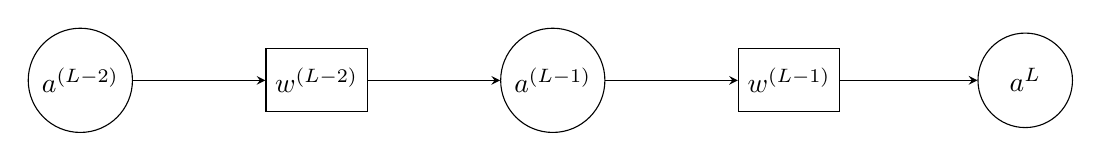
\begin{tikzpicture}[x=1.5cm, y=1.5cm,  >=stealth]
        \tikzstyle{unit}=[draw,shape=circle,minimum size=1.2cm]
        \tikzstyle{weight} =[draw, shape=rectangle, minimum size=.8cm]

        \node[unit](I) at (0, 2){$a^{(L-2)}$};
        \node[weight](w1) at (2,2){$w^{(L-2)}$};
        \node[unit](H) at (4, 2){$a^{(L-1)}$};
        \node[weight](w2) at (6,2){$w^{(L-1)}$};
        \node[unit](O) at (8, 2){$a^L$};
        
        \draw[->] (I) -- (w1);
        \draw[->] (w1) -- (H);
        \draw[->] (H) -- (w2);
        \draw[->] (w2) -- (O);
        
        \end{tikzpicture}
	\caption[]{Einfaches Neuronal Network mit nur einem Neuron pro Layer}
    \label{fig:simpleNetwork}
    Quelle: Eigene Darstellung, 2020
\end{figure}


\begin{figure}[H]
    \centering
    \begin{tikzpicture}[x=1.5cm, y=1.5cm,  >=stealth]
        \tikzstyle{unit}=[draw,shape=circle,minimum size=1.2cm]
        \tikzstyle{weight} =[draw, shape=rectangle, minimum size=.8cm]

        \node[weight](w) at (0, 2){$w^{(L-1)}$};
        \node[weight](a) at (0, 1){$a^{(L-1)}$};
        \node[weight](b) at (0,0){$b^{(L-1)}$};
        \node[weight](z) at (2, 1){$z^{(L)}$};
        \node[weight](aL) at (4,1){$a^{(L)}$};
        \node[unit](c) at (6,1){$C$};
        \node[weight](y) at (6,0){$y$};

        \draw[->] (w) -- (z);
        \draw[->] (a) -- (z);
        \draw[->] (b) -- (z);
        \draw[->] (z) -- (aL);
        %\path [line] (aL) -- node [text width=2.5cm,midway,above ]{$\hat{y}$} (c);
        \draw[->] (aL) -> node [text width=2.5cm,midway,above,align=center ] {$\hat{y}$} (c);

        \draw[->] (y) -- (c);

        \end{tikzpicture}
    \caption[]{Vereinfachte Darstellung der Einflüsse auf die Verlustfunktion}
    \label{fig:unfoldedCost}
    Quelle: Eigene Darstellung, 2020
\end{figure}

Stellt man sich ein möglichst einfaches \ac{NN} mit Hidden Layer vor, erhält man das in Abbildung \ref{fig:simpleNetwork} dargestellte \ac{NN}. Dieses enthält pro Layer nur ein Neuron. $L$ stellt hierbei die Anzahl der Layer im Netzwerk da. Die einzelnen Layer werdem dementsprechend durchnummeriert, wobei die Ziffer des Output Layers gleich $L$ ist und mit jeden weiteren Schritt nach links Eins subtrahiert wird. In dem \ac{NN} aus Abbildung \ref{fig:simpleNetwork} ergeben sich somit die Kennziffern $L = 3$ für den Output Layer, $L-1 = 2 $ für den Hidden Layer und $L-2 = 1 $ für den Input LAyer

In Abbildung \ref{fig:unfoldedCost} sind die Einflüsse auf die Verlustfunktion für den Output Layer $C$ dargestellt.  Für eine bessere Übersichtlichkeit wurde auf die Indizes für eine zuordnung der Neuronen innerhalb des \ac{NN} verzichtet.

Es ist zu erkennen, dass die Eingänge in die gewichtete Summe $z^{(L)}$ sich aus den Gewichten $w^{(L-1)}$, der Aktivierung $a^{(L-1)}$ und dem Bias $b^{(L-1)}$ zusammensetzten. Das Ergebnis von $z^{(L)}$ wird anschließend in die Aktivierungsfunktion a gegeben, wodurch wir die Aktivierung des Output Layers $a^{(L)}$ erhalten. Aus diesem und dem tatsächlich erwarteten Wert - $t$ - wird abschließend die Verlustfunktion gebildet. 
